% !TeX root = ../report_project_2stage_OTA.tex

\section{Characterization}

\subsection{Slew-Rate Verification}

The final OTA is configured as a unity-gain follower and driven by a
$0.45$--$0.75~\mathrm{V}$ input step with $C_L=4~\mathrm{pF}$.
The slew rate is estimated from the average 20--80\% output-transition
slope, with the local derivative around the transition midpoint used as
an additional check.

The simulated 20--80\% slopes are
\[
\boxed{SR_{\mathrm{rise}}=0.549~\mathrm{V}/\mu\mathrm{s}},
\qquad
\boxed{SR_{\mathrm{fall}}=0.469~\mathrm{V}/\mu\mathrm{s}}.
\]
The corresponding midpoint derivatives are
\[
SR_{\mathrm{rise,mid}}=+0.558~\mathrm{V}/\mu\mathrm{s},
\qquad
SR_{\mathrm{fall,mid}}=-0.429~\mathrm{V}/\mu\mathrm{s}.
\]
The two measurements reflect slightly different regions of each
transition; in particular, the falling edge is not perfectly linear.
The 20--80\% values are retained as the reported slew rates.

A first-order first-stage current-limited estimate gives
\[
\frac{I_{\mathrm{tail,1}}}{C_M}
\approx\frac{0.5~\mu\mathrm{A}}{736.44~\mathrm{fF}}
\approx0.68~\mathrm{V}/\mu\mathrm{s}.
\]
The simulated large-signal response also depends on current
redistribution, second-stage dynamics, the output load, and transistor
parasitics; this simple estimate is therefore not an exact prediction.

\subsection{Saturation and Headroom Criterion}

The usable input and output voltage ranges are assessed using both
compact-model operating-point information and a practical
source-to-drain headroom criterion, rather than relying exclusively on
an inversion-region flag.

At $27^\circ\mathrm{C}$, the thermal voltage is
\[
U_T=\frac{kT}{q}\approx25.9~\mathrm{mV}.
\]
For this first-order headroom assessment, a conservative screening
criterion is chosen as
\[
\boxed{|V_{DS}|\gtrsim4U_T\approx0.10~\mathrm{V}}.
\]
This is an engineering approximation for the present low-current design,
not a universal saturation condition for every MOS operating point.
Final usable ranges must also be checked against bias-current
regulation, gain, and the full compact-model behavior.

\subsection{Input Common-Mode Range}

The first stage uses the PMOS input pair \texttt{PDIFF\_N/P}, biased by
\texttt{PTAIL\_1} and loaded by the diode-connected NMOS mirror
\texttt{NLOAD\_0/1}.

\subsubsection{Lower ICMR Limit}

The PMOS pair requires sufficient source-to-drain headroom,
\[
V_{SD,\mathrm{PDIFF}}\gtrsim4U_T.
\]
With
\[
V_{S,\mathrm{PDIFF}}=V_{CM}+V_{SG,\mathrm{PDIFF}}
\]
and the diode-connected load approximately fixing one input-device
drain voltage at $V_{GS,\mathrm{NLOAD0}}$, the lower limit is estimated as
\[
V_{CM,\min}\approx
V_{GS,\mathrm{NLOAD0}}+4U_T-V_{SG,\mathrm{PDIFF}}.
\]
For single-supply operation, the practical range is additionally
bounded by ground:
\[
V_{CM,\min,\mathrm{usable}}\gtrsim0~\mathrm{V}.
\]

\subsubsection{Upper ICMR Limit}

At large $V_{CM}$, the first-stage PMOS source device
\texttt{PTAIL\_1} becomes limiting:
\[
V_{SD,\mathrm{PTAIL1}}=
V_{DD}-\left(V_{CM}+V_{SG,\mathrm{PDIFF}}\right)
\gtrsim4U_T.
\]
Thus,
\[
\boxed{V_{CM,\max}\approx
V_{DD}-V_{SG,\mathrm{PDIFF}}-4U_T}.
\]

The earlier numerical ICMR estimate was based on operating-point
voltages from the initial transistor sizing. Since \texttt{NLOAD\_0/1}
were substantially resized, those voltages have not been reused here.
A numerical ICMR specification for the final sizing requires an updated
operating-point extraction and common-mode sweep; the equations above
are topology-based design estimates only.

\subsection{Output Common-Mode Range}

The second stage comprises the PMOS current source \texttt{PTAIL\_2}
and the active NMOS common-source device \texttt{NLOAD\_2}.
Assuming the same first-order $4U_T$ headroom criterion at each output
device gives
\[
V_{\mathrm{out,min}}\approx4U_T\approx0.10~\mathrm{V},
\]
\[
V_{\mathrm{out,max}}\approx V_{DD}-4U_T
\approx1.70~\mathrm{V}
\quad(V_{DD}=1.8~\mathrm{V}).
\]
The resulting topology-based nominal estimate is
\[
\boxed{\mathrm{OCMR}_{\mathrm{est.}}\approx
0.10\text{--}1.70~\mathrm{V}}.
\]
This is a headroom estimate, not a final measured output-swing
specification. A dedicated large-signal sweep on the final device
sizing is required to verify current regulation, distortion, and
usable output limits.

\subsection{Positive-Supply Rejection}

% VERIFY BEFORE RELEASE: record the final PSRR testbench C_L here.
The final OTA is simulated as a unity-gain follower around a
$0.6~\mathrm{V}$ reference, with $V_{DD}=1.8~\mathrm{V}$ and a
normalized small-signal supply excitation of $1~\mathrm{V}$.
The positive-supply rejection ratio is calculated as
\[
PSRR_+(f)=20\log_{10}\left|\frac{v_{DD}(f)}{v_{\mathrm{out}}(f)}\right|.
\]

\begin{table}[ht]
    \centering
    \caption{Final nominal positive-supply rejection from the
    regenerated PSRR testbench.}
    \label{tab:psrr_plus}
    \begin{tabular}{lc}
        \hline
        Frequency & $PSRR_+$ \\
        \hline
        1 Hz     & 99.88 dB \\
        1 kHz    & 99.86 dB \\
        100 kHz  & 84.73 dB \\
        1 MHz    & 59.02 dB \\
        10 MHz   & 49.85 dB \\
        \hline
    \end{tabular}
\end{table}

At low frequency, the final nominal result is approximately
\[
\boxed{PSRR_+(1~\mathrm{kHz})=99.86~\mathrm{dB}}.
\]
As frequency increases, the declining feedback gain and parasitic
supply-to-output coupling reduce rejection. The load-dependent
$2$-pF/$4$-pF comparison from the original sizing is intentionally not
reproduced here, as it was not rerun for the final circuit.

\subsection{Noise}

The final OTA is characterized as a unity-gain follower at
$V_{DD}=1.8~\mathrm{V}$, with the input reference at $0.6~\mathrm{V}$
and $C_L=2~\mathrm{pF}$. The integrated noise interval is
\[
1~\mathrm{Hz}\le f\le1~\mathrm{MHz}.
\]
The final integrated results are
\[
\boxed{v_{n,\mathrm{out,rms}}=120.27~\mu\mathrm{V}},
\qquad
\boxed{v_{n,\mathrm{in,rms}}=134.66~\mu\mathrm{V}}.
\]
Compared with the initial sizing ($175.53~\mu\mathrm{V}$ output RMS
and $191.09~\mu\mathrm{V}$ input RMS), these represent reductions of
approximately 31.5\% and 29.5\%, respectively.

Device-level integration identifies the first-stage NMOS mirror as the
largest output-noise contributor. Squaring each device's integrated
RMS contribution and dividing by the squared total output noise gives
\[
\underbrace{38.0\%}_{\texttt{NLOAD\_1}}+
\underbrace{34.8\%}_{\texttt{NLOAD\_0}}
\approx72.8\%.
\]
The two PMOS input devices jointly contribute approximately 20.3\%
of the output-noise power; the compensation resistor contributes about
3.8\% and \texttt{NLOAD\_2} approximately 1.5\%. Other devices
account for the remainder.

The load-mirror contribution has decreased from approximately 87.6\%
in the original circuit to 72.8\% with the selected larger NMOS
mirror devices. The mirror remains the dominant noise source, but the
PMOS input pair is no longer negligible. In this final simulation the
integrated NMOS mirror noise contains a substantial channel thermal
component, explaining why additional area increases need not produce
a proportional reduction in total integrated noise.

The noise ranking separately reports device totals and their internal
mechanisms (e.g. channel and $1/f$ noise); those entries must not be
summed together as independent device contributions.

\subsection{PVT Analysis}

The final transistor-level OTA was evaluated over five process corners:
SS, SNFP (slow NMOS/fast PMOS), TT, FNSP (fast NMOS/slow PMOS), and FF.
Each was combined with
\[
V_{DD}\in\{1.62,\ 1.80,\ 1.98\}~\mathrm{V}
\quad\text{and}\quad
T\in\{-40,\ 27,\ 125\}~^\circ\mathrm{C},
\]
for 45 operating conditions in total. The sweep used the maximum
specified load, $C_L=4~\mathrm{pF}$, and the selected physical
compensation network,
\[
C_M=736.44~\mathrm{fF},\qquad R_M=180~\mathrm{k}\Omega.
\]
The reported metrics are low-frequency open-loop gain, unity-gain
frequency, phase margin, gain margin, quiescent current, and PSRR at
$1~\mathrm{kHz}$.

At TT, $V_{DD}=1.8~\mathrm{V}$ and $T=27^\circ\mathrm{C}$, the
$4$-pF results are
\[
A_0=89.73~\mathrm{dB},\qquad
f_{\mathrm{UGF}}=1.0676~\mathrm{MHz},
\]
\[
PM=74.98^\circ,\qquad GM=17.9~\mathrm{dB},
\]
with $I_Q=4.001~\mu\mathrm{A}$ and
$PSRR_+(1~\mathrm{kHz})=99.86~\mathrm{dB}$.

% AUTO-GENERATED -- DO NOT EDIT

\begin{table}[ht]
    \centering
    \caption{Main electrical performance over the
    45-point PVT matrix at $C_L=4~\mathrm{pF}$.}
    \label{tab:pvt_summary}

    \begin{tabular}{lccc}
        \hline
        Metric & Nominal & Worst PVT & Worst condition \\
        \hline

        DC gain &
        89.7 dB &
        87.6 dB &
        FNSP / $+125^\circ\mathrm{C}$ / 1.62 V \\

        UGF &
        1068 kHz &
        828 kHz &
        FNSP / $+125^\circ\mathrm{C}$ / 1.62 V \\

        Phase margin &
        75.0$^\circ$ &
        64.7$^\circ$ &
        SS / $+125^\circ\mathrm{C}$ / 1.62 V \\

        Gain margin &
        17.9 dB &
        13.8 dB &
        SNFP / $-40^\circ\mathrm{C}$ / 1.98 V \\

        Supply current &
        4.00 $\mu$A &
        4.05 $\mu$A &
        FNSP / $+125^\circ\mathrm{C}$ / 1.98 V \\

        PSRR$^+$ @ 1 kHz &
        99.9 dB &
        53.3 dB &
        SNFP / $-40^\circ\mathrm{C}$ / 1.62 V \\

        \hline
    \end{tabular}
\end{table}


The minimum DC gain is $87.63~\mathrm{dB}$ (FNSP,
$125^\circ\mathrm{C}$, $1.62~\mathrm{V}$). The minimum phase margin is
$64.69^\circ$ (SS, $125^\circ\mathrm{C}$, $1.62~\mathrm{V}$), while
the minimum gain margin is $13.76~\mathrm{dB}$ (SNFP,
$-40^\circ\mathrm{C}$, $1.98~\mathrm{V}$).
Thus, all 45 cases meet the hard criteria
\[
\boxed{A_0\ge80~\mathrm{dB},\quad
PM\ge60^\circ,\quad GM>10~\mathrm{dB}}.
\]
The UGF ranges from $827.8~\mathrm{kHz}$ to
$1.4652~\mathrm{MHz}$ across PVT at $C_L=4~\mathrm{pF}$. The
nominal-bandwidth target of $1~\mathrm{MHz}$ was defined for
$C_L=2~\mathrm{pF}$, for which the final TT simulation reaches
$1.1838~\mathrm{MHz}$.

The supply-current range is $3.787$--$4.050~\mu\mathrm{A}$, and the
lowest simulated PSRR at $1~\mathrm{kHz}$ is $53.28~\mathrm{dB}$
(SNFP, $-40^\circ\mathrm{C}$, $1.62~\mathrm{V}$). This significant
corner sensitivity is reported separately from the gain and stability
requirements rather than being described as invariant.

As defined in Section~2.4, the external $500~\mathrm{nA}$ bias source
is ideal and fixed; the results therefore exclude variability of a
physical bias-current generator.

\subsection{Monte Carlo Analysis}

Monte Carlo analysis was used to quantify the effects of the SKY130
statistical process and local-mismatch models on the input-referred
offset $V_{OS}$ and low-frequency open-loop gain $A_0$.
Both variation mechanisms were enabled. The final campaign used
300 independent samples per combination of
\[
V_{DD}\in\{1.62,\ 1.80,\ 1.98\}~\mathrm{V},\qquad
T\in\{-40,\ 27,\ 125\}~^\circ\mathrm{C},
\]
for a total of 2700 simulations, at $C_L=4~\mathrm{pF}$.
The offset is input-referred using the unity-follower DC solution,
with a finite-gain correction using the sampled $A_0$; gain is
extracted from the low-frequency AC response of the same randomized
sample. These results describe the available open-source statistical
models and are not claimed to be foundry-qualified sign-off data.

\subsubsection{Offset-Driven Sizing Iterations}

The initial input-referred offset standard deviation at
$1.8~\mathrm{V}$ and $27^\circ\mathrm{C}$ was
$6.125~\mathrm{mV}$. This motivated an iterative increase of the
first-stage NMOS mirror-load area while approximately preserving its
unit-device $W/L$ ratio. The two load transistors were initially much
smaller in gate area than the PMOS input pair.

\begin{table}[ht]
    \centering
    \caption{Offset optimization at $V_{DD}=1.8~\mathrm{V}$ and
    $T=27^\circ\mathrm{C}$ ($N=300$ for each design). Transistor
    $W/L$ is given in $\mu\mathrm{m}/\mu\mathrm{m}$; the final row
    uses the retuned Miller network.}
    \label{tab:mc_sizing_iterations}
    \small
    \begin{tabular}{lllrr}
        \hline
        Design & \texttt{NLOAD\_0/1} & \texttt{NLOAD\_2}
        & $\sigma(V_{OS})$ & $3\sigma(V_{OS})$ \\
        \hline
        Initial & $0.6/2$, $m=1$ & $0.6/2$, $m=12$
        & 6.125 mV & 18.37 mV \\
        Iter. 1 & $2.4/8$, $m=1$ & $0.6/2$, $m=12$
        & 1.448 mV & 4.34 mV \\
        Iter. 2 & $3.6/12$, $m=1$ & $3.6/6$, $m=6$
        & 1.195 mV & 3.58 mV \\
        Iter. 3 & $3.6/12$, $m=1$ & $3.6/2$, $m=2$
        & 1.163 mV & 3.49 mV \\
        Iter. 4 & $4.2/14$, $m=1$ & $3.6/2$, $m=2$
        & 1.177 mV & 3.53 mV \\
        Final & $3.6/12$, $m=1$ & $3.6/2$, $m=2$
        & 1.109 mV & 3.33 mV \\
        \hline
    \end{tabular}
\end{table}

Increasing the mirror-load area initially reduced the offset
standard deviation by a factor of approximately four, broadly
consistent with the first-order matching trend
\[
\sigma_{\mathrm{mismatch}}\propto\frac{1}{\sqrt{WL}}.
\]
Changing \texttt{NLOAD\_2} separately recovered stability by limiting
the gate capacitance at the high-impedance first-stage output node
\texttt{out\_s1}. This device is an \emph{active} second-stage NMOS,
not a non-functional layout dummy. In the selected sizing,
\[
\frac{m_2(W/L)_2}{m_{0,1}(W/L)_{0,1}}=
\frac{2(3.6/2)}{1(3.6/12)}=12.
\]
This is an effective geometric $W/L$ ratio, not a guarantee of an
identical current-density relationship between devices of different
channel length.

The subsequent Iteration 4 produced no statistically significant
reduction in offset dispersion and required more mirror area.
Iteration 3 was therefore retained as the transistor-sizing baseline;
Miller-compensation optimization subsequently produced the selected
final circuit. The small difference between the Iteration-3 and final
Monte Carlo estimates should not be ascribed solely to the compensation
change because the results come from independent 300-sample datasets.

\subsubsection{Final Statistical Performance}

\begin{table}[H]
\centering
\caption{Monte Carlo summary for process and mismatch variations.}
\label{tab:mc_summary}
\small
\begin{tabular}{ccrrrr}
\toprule
$V_{DD}$ [V] & $T$ [$^\circ$C] & $\mu(V_{OS})$ [mV] & $\sigma(V_{OS})$ [mV] & $\mu(A_0)$ [dB] & $\sigma(A_0)$ [dB] \\
\midrule
1.62 & -40 & +0.31 & 1.24 & 89.04 & 0.129 \\
1.80 & -40 & +0.25 & 1.24 & 89.46 & 0.180 \\
1.98 & -40 & +0.30 & 1.25 & 89.62 & 0.180 \\
1.62 & 27 & +0.20 & 1.28 & 89.83 & 0.073 \\
1.80 & 27 & +0.04 & 1.11 & 90.04 & 0.070 \\
1.98 & 27 & +0.19 & 1.15 & 90.21 & 0.080 \\
1.62 & 125 & +0.10 & 1.14 & 89.31 & 0.054 \\
1.80 & 125 & +0.11 & 1.15 & 89.56 & 0.061 \\
1.98 & 125 & +0.13 & 1.20 & 89.76 & 0.064 \\
\bottomrule
\end{tabular}
\end{table}


At nominal supply and temperature, the final offset distribution has
\[
\boxed{\mu(V_{OS})=+0.0396~\mathrm{mV},\qquad
\sigma(V_{OS})=1.1089~\mathrm{mV}},
\]
so $3\sigma(V_{OS})=3.327~\mathrm{mV}$. This is an 81.9\%
reduction in offset standard deviation relative to the initial design.
The final mean offset is small compared with the spread and the
distribution must not be summarized by its mean alone.

\begin{figure}[H]
    \centering
    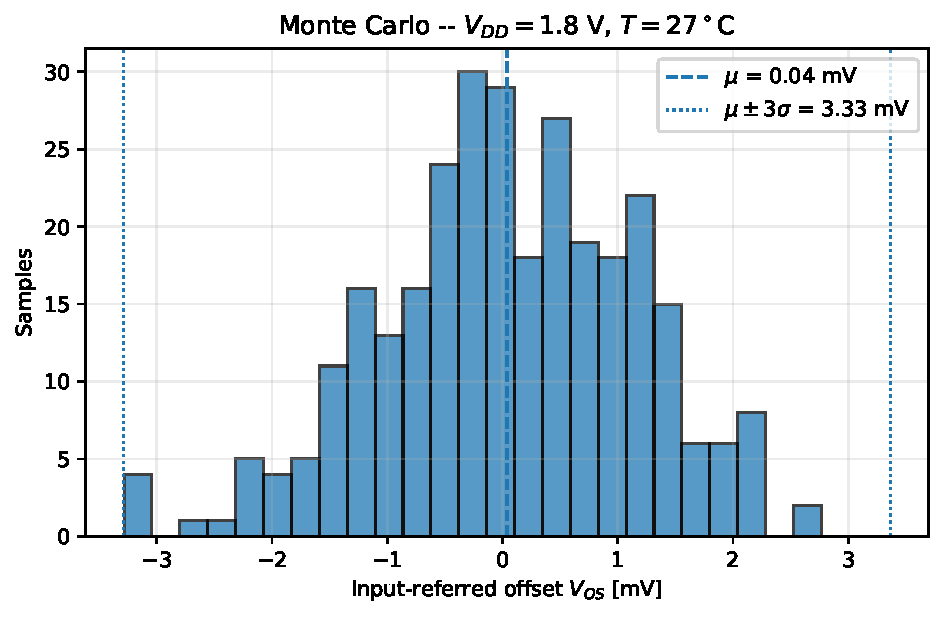
\includegraphics[width=0.78\linewidth]
    {figures/montecarlo/mc_vos_nominal.pdf}
    \caption{Final input-referred offset distribution at
    $V_{DD}=1.8~\mathrm{V}$ and $T=27^\circ\mathrm{C}$ ($N=300$).}
    \label{fig:mc_vos}
\end{figure}

The corresponding nominal gain distribution has
\[
\boxed{\mu(A_0)=90.04~\mathrm{dB},\qquad
\sigma(A_0)=0.070~\mathrm{dB}}.
\]
The nominal lower $\mu-3\sigma$ estimate is approximately
$89.83~\mathrm{dB}$, well above the $80~\mathrm{dB}$ target.
The deterministic TT gain of $89.73~\mathrm{dB}$ need not coincide
exactly with the mean of the randomized ensemble.

\begin{figure}[H]
    \centering
    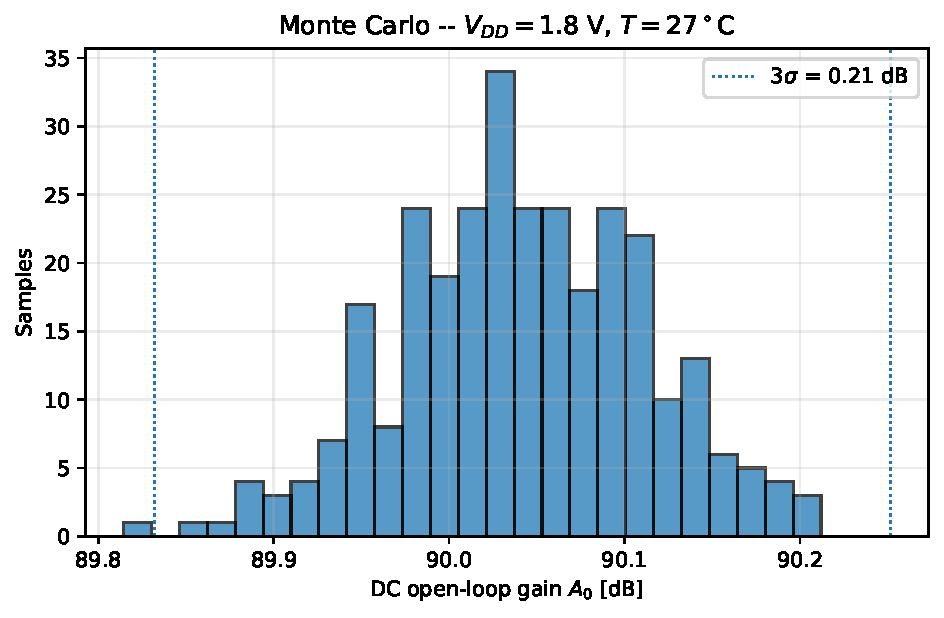
\includegraphics[width=0.78\linewidth]
    {figures/montecarlo/mc_gain_nominal.pdf}
    \caption{Final low-frequency open-loop gain distribution at
    $V_{DD}=1.8~\mathrm{V}$ and $T=27^\circ\mathrm{C}$ ($N=300$).}
    \label{fig:mc_gain}
\end{figure}

Across the nine conditions, the maximum observed offset standard
deviation is $1.277~\mathrm{mV}$, corresponding to
$3\sigma=3.831~\mathrm{mV}$ at $V_{DD}=1.62~\mathrm{V}$ and
$T=27^\circ\mathrm{C}$. The largest absolute mean offset is
$0.313~\mathrm{mV}$ at $1.62~\mathrm{V}$ and $-40^\circ\mathrm{C}$.
For a two-sided absolute-offset estimate, the worst value of
$|\mu|+3\sigma$ across these conditions is approximately
$4.06~\mathrm{mV}$ at $1.98~\mathrm{V}$ and $-40^\circ\mathrm{C}$.

The minimum gain-ensemble mean is $89.04~\mathrm{dB}$ and the most
conservative lower $\mu-3\sigma$ estimate among the nine conditions
is approximately $88.65~\mathrm{dB}$, above the gain requirement.
The optimization objective of approximately $3~\mathrm{mV}$ at
$3\sigma$ was not fully met (even at nominal conditions), despite the
substantial improvement. This trade-off is reported explicitly instead
of treating a statistical target as achieved.
